\chapter{On the SRT Algorithm}\label{Chapter_SRT}

The SRT algorithm was independently developed around 1958 by three researchers: Sweeney (IBM), Robertson (University of Illinois) and Tocher (Imperial College London).
The first letter of their surnames form the name of the algorithm.
In the area of slow division algorithms, which are able to produce $k$ exact digits of the quotient per clock cycle, it is currently the most used. 

It became famous in 1990 because of a bug in the floating point division unit of the Pentium 486DX processor .
At the end of this appendix, the reader will have the instruments needed to understand what was wrong with their implementation.
Before that, we need to start understanding how is it possible to divide binary numbers, in order to gradually introduce the ideas behind SRT.

The following material comes from \cite{ruiz2021arithmetic} and \cite{parhami2010computer}. 

\section{Simple division algorithms}

In division, given a dividend $D$ on $m$ bits and a divisor $d$ on $n$ bits, we want to find two unsigned binary numbers $Q$ and $R$, with $R < d$, such that 

\[
    D = Q \cdot d + R
\]

As it is widely known, before diving into a division we need to check that $d \neq 0$, otherwise the above expression would make no sense.
In the context of binary numbers, we also need to check that the final quotient can be expressed on $n$ bits (same size of the divisor). 
This condition is not always satisfied, so we need more constraints.

We want $Q < 2^n$ and, since it still has to be true that $R < d$, we obtain the following inequality:

\[
    D = Q \cdot d + R \leq (2^n - 1) \cdot d + d = 2^n \cdot d
\]

This condition has to be checked before the division, otherwise the quotient will overflow and its representation will be wrong. 

\subsection{Restoring algorithm}

The simplest algorithm we can think of is the \textit{restoring algorithm} as it is identical to the one we learnt during elementary school.
We compute one digit $q_i$ of the quotient $Q$ at a time (most significant bit first) by looking at the most significant digits of the current remainder.
In the binary case, $q_i \in \{0, 1\}$, so what we need to check is whether $d$ is greater or less than the $N/2$ most significant digits of the current remainder $A$. 
    
In hardware we cannot guess as we do on paper, so we try to perform a subtraction between $A$ and $2^{N/2}\cdot d$ ($d$ is left-shifted by $2^{N/2}$ to subtract it from $A$'s most significant digits, due to A being twice as long as $d$): if the result is positive, then the correct digit of the quotient $q_i$ is 1, otherwise it is 0.

The following code block is an implementation of the above algorithm in C++, using a library defined specifically to simulate the behaviour of VHDL's \texttt{std\_logic\_vector} type.
It will be used later on for the same purpose.


\begin{lstlisting}[language=C++]
std::pair<SLV::std_logic_vector, SLV::std_logic_vector> 
Division::restoring_division
(SLV::std_logic_vector& dividend, SLV::std_logic_vector&  divisor){
 
    int N = divisor.size;

    if(dividend.to_base_10() >= (divisor.to_base_10() << N/2))
        throw std::invalid_argument();    

    SLV::std_logic_vector R(N/2);
    SLV::std_logic_vector Q(N/2 + 1);
    SLV::std_logic_vector A(N + 1);
    SLV::std_logic_vector B(N + 1);

    A = SLV::std_logic_vector(1) & 
        dividend;

    B = SLV::std_logic_vector(1) & 
        divisor.extract(N/2 - 1, 0)  & 
        SLV::std_logic_vector(N);

    for(int i = N/2; i >= 0; i--){         
        A = A - B;
        if(A.get_msb() == 0)
            Q.set(i),
            A = A << 1;
        else
            Q.reset(i),
            A = (A + B) << 1;
    }

    R = A.extract(N, N/2 + 1);
    Q = Q.extract(N/2 - 1, 0);

    return std::pair<SLV::std_logic_vector, SLV::std_logic_vector>
    (Q, R);
}
\end{lstlisting}

It is clear from the code that, in order to decide which is the current digit of the quotient $q_i$ and calculate the current remainder, we first need to perform $A - B$ : since in an hardware implementation this difference is stored in a register that we first write to and then read from, to compute one digit of the quotient we need $2$ clock cycles.

\begin{figure}
    \centering
    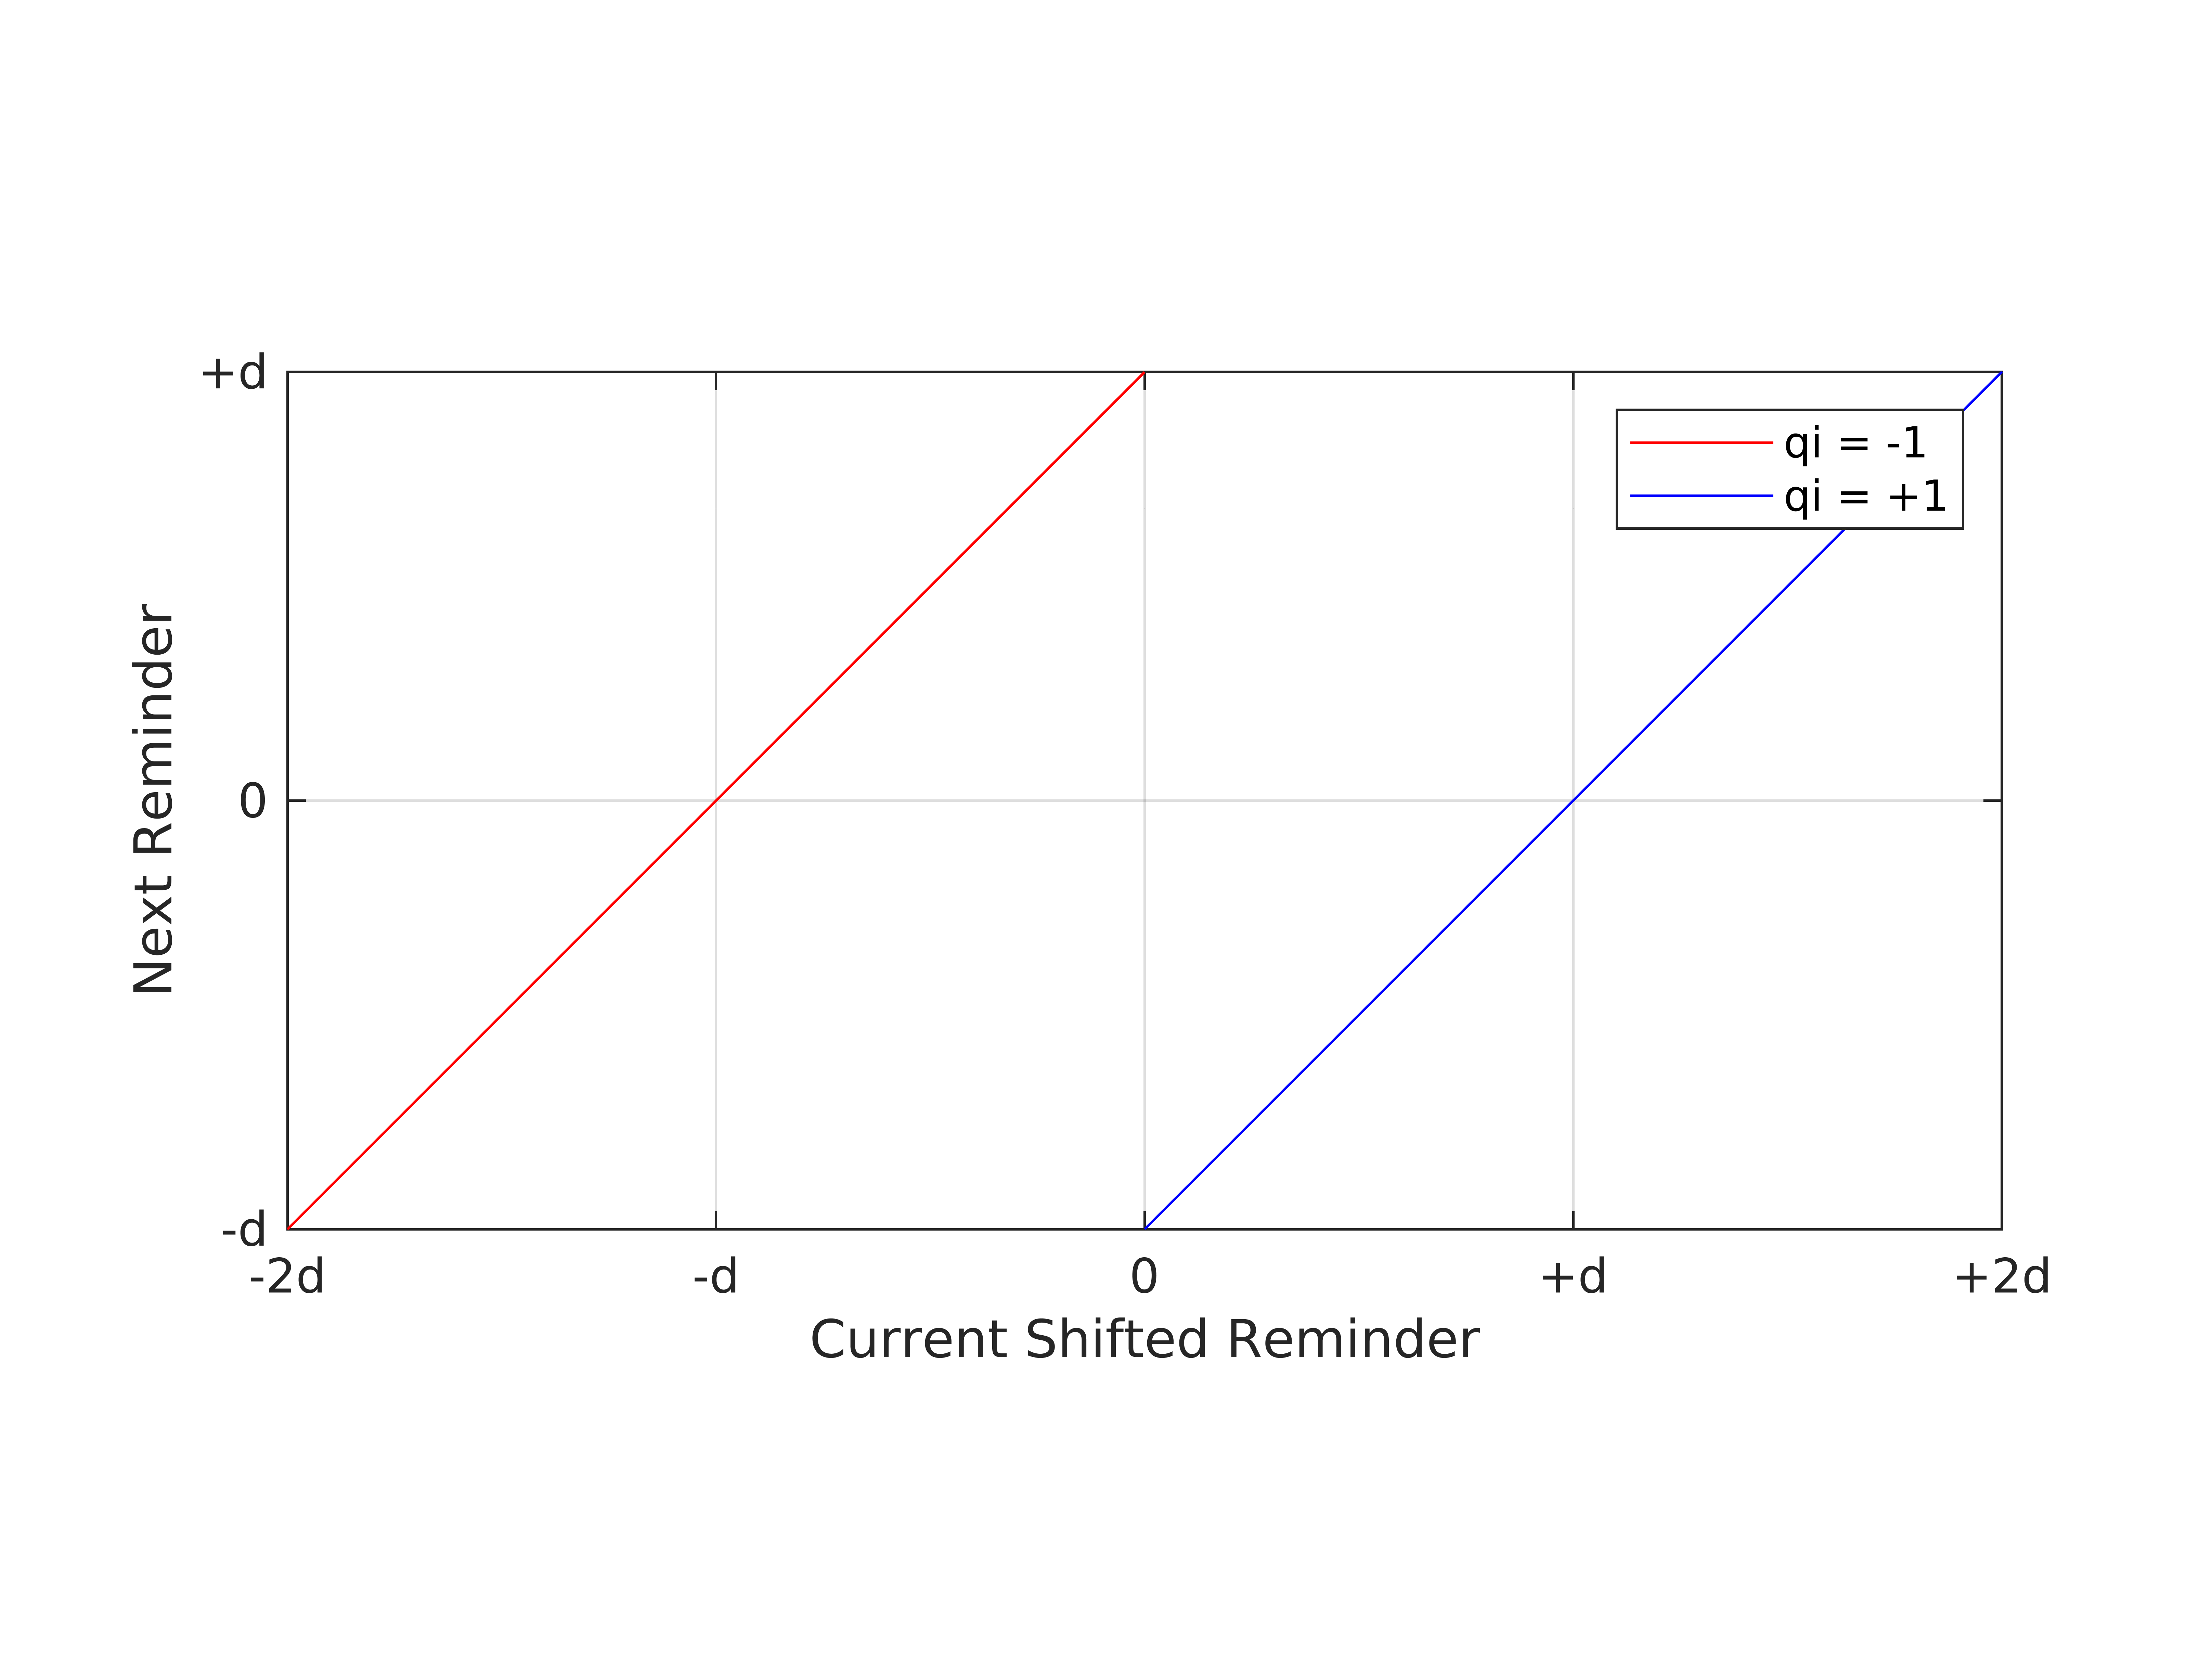
\includegraphics[width=150mm]{images/non_rest.png}
    \caption{Non restoring division: operation to perform at each cycle}
    \label{fig:non_rest}
\end{figure}

\subsection{Non-restoring algorithm}
The \textit{non-restoring algorithm} solves this problem: as we can see from \autoref{fig:non_rest}, depending on the current value of the shifted remainder we either subtract or add $2^{N/2} \cdot d$  and choose the digit of the quotient based on the sign of the current remainder $A$.

Here is an implementation of the algorithm: 

\begin{lstlisting}[language=C++]
std::pair<SLV::std_logic_vector, SLV::std_logic_vector> 
Division::non_restoring_division
(SLV::std_logic_vector& dividend, SLV::std_logic_vector & divisor){
    
    int N = divisor.size;

    if(dividend.to_base_10() >= (divisor.to_base_10() << N/2))
        throw std::invalid_argument();    

    SLV::std_logic_vector Q(N/2 + 1);
    SLV::std_logic_vector R(N/2);
    SLV::std_logic_vector A(N + 2);
    SLV::std_logic_vector B(N + 2);

    A = SLV::std_logic_vector(2) &
        dividend;
    
    B = SLV::std_logic_vector(2)  & 
        divisor.extract(N/2 - 1, 0) &
        SLV::std_logic_vector(N/2);

    for(int i = N/2; i >= 0; i--){
        if(A.get_msb() == 0)
            Q.set(i),
            A = (A - B) << 1;
        else
            Q.reset(i),
            A = (A + B) << 1;
    }

    Q = Q - Q.complement();

    if(A.get_msb() == 1)
        Q = Q - 1,
        A = ((A >> 1) + B) << 1;

    R = A.extract(2 * N/2, N/2 + 1);
    Q = Q.extract(N/2 - 1, 0); 

    return std::pair<SLV::std_logic_vector, SLV::std_logic_vector>
    (Q, R);
}
\end{lstlisting}

In this algorithm, we can see something which will be very useful in the SRT division: a non-standard encoding of the digits of the quotient. 
Instead of using $\{0, 1\}$, at each clock cycle we choose $q_i$ in $\{-1, 1\}$. 
The value of a number that uses this special digit set can be computed as $\sum a_i \cdot 2^i$ where $a_i \in \{-1, 1\}$.

At the end of the algorithm, we need to re-code the quotient to the more standard $\{0, 1\}$ digit set. 
This is not complicated, depending on the way we implement the $\{-1, 1\}$ encoding.
For instance, we can represent -1 as a 0 in the quotient register, and then compute $Q = Q - \bar{Q}$. 
This is what happens in the example above.
Another possibility is to use two registers, $Q$ and $C$: we set $Q_i$ to 1 when the final quotient's digit $q_i$ is 1, else we set $C_i$, and then compute $Q = Q - C$.
Later on we will see that this computation can be also done \textit{on the fly}.

Another issue is that, by accepting to have remainders which are not correct, we may end up with a negative remainder once all of the quotient's digits have been calculated.
In this case a further correction is required: we decrease $Q$ by one and add the shifted divisor to the remainder.
Again, this final correction is shown in the code.

The loop now requires $N/2$ or $N/2+1$ clock cycles (depends whether the quotient and remainder need to be corrected at the end), since we can set one digit of the quotient and compute the remainder at the same time. 

\section{The SRT division}

It is difficult to use one of the previously analysed approaches to design a division process with a radix higher than 2: an algorithm in radix $2^k$ is able to compute $k$ digits of the final result at each iteration, so the higher the radix the faster the result is generated. 

The SRT algorithm tries to solve this problem by requiring $d \in \left[ \frac{1}{2}, 1\right)$ before the division can be performed: this is particularly simple in binary representation because it means that $d$'s most significant bit has to be 1.
It should be noted that, should a normalisation take place, the dividend $D$ will have to be normalised too.
It may be useful to recall that, given a fixed-point fractional binary number $0.a_{-1}a_{-2}...a_{-n}$ we can compute its value in base ten using the expression 

\[
    A = \sum_{i=1}^{n} a_{-i} \cdot 2^{-i}
\]

For example, the decimal conversion of $0.101$ is $1 \cdot \frac{1}{2}+0 \cdot \frac{1}{4}+ 1 \cdot \frac{1}{8} = \frac{5}{8}$.
The integer part, if different from 0, can be calculated using the standard binary-to-decimal conversion method.
This constraint on the operands is particularly convenient for IEEE-754 floating point numbers, since their mantissa is already represented as $1.xxxx...$ (so it just needs to be shifted one position to the right to be normalised).
However, the algorithm (and its implementation) can be used for signed/unsigned integer numbers as well, provided that we normalise them and then adjust the result of the division.

\subsection{Radix-2 algorithm}

Knowledge of the radix-2 version is preliminary for the radix-4, as the basic principles are the same for both. 

\begin{figure}
    \centering
    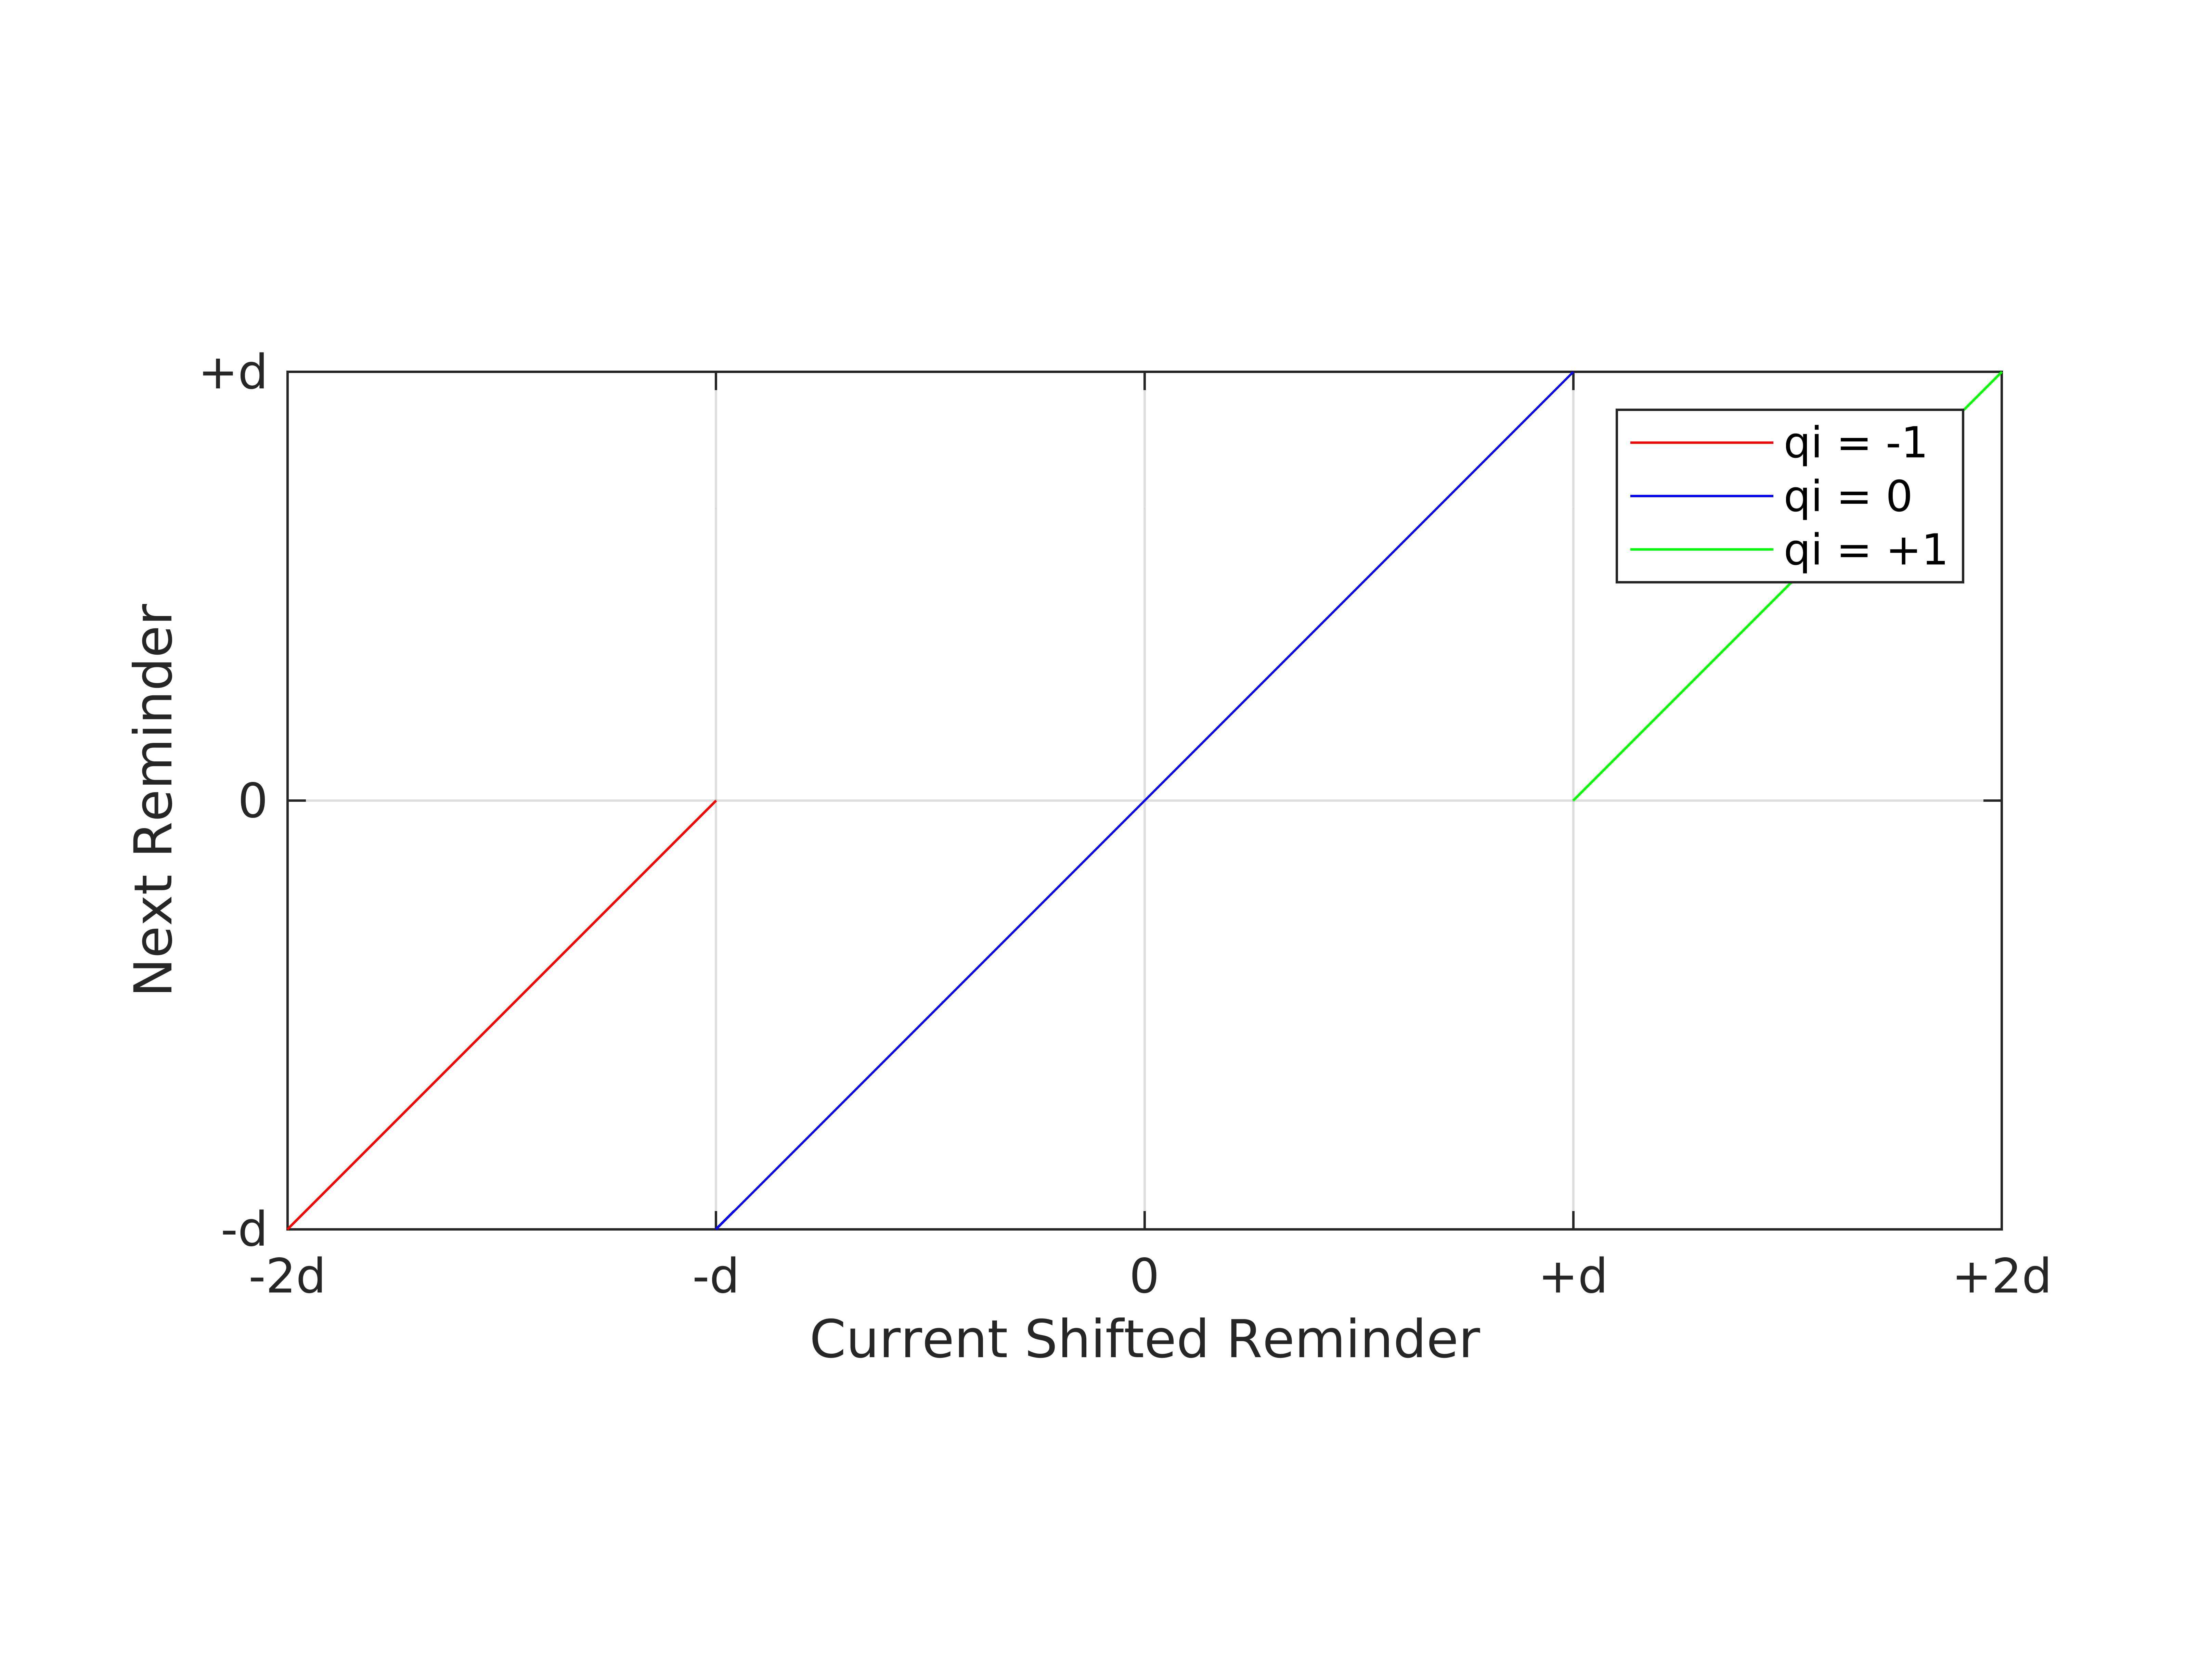
\includegraphics[width=100mm]{images/srt_2_plot_1.png}
    \caption{SRT: operation to perform at each cycle without normalisation}
    \label{fig:srt_2_plot_1}
\end{figure}

We want to work with the $\{-1, 0, 1\}$ digit set. 
\autoref{fig:srt_2_plot_1}  shows how to compute the next remainder and quotient digit $q_i$ starting from the current remainder and using the above digit set: this graph is not very useful, as it requires comparing the value of the current remainder both with $d$ and $-d$ before knowing what to do, which is way more complex than checking the remainder's most significant bit. 

This is where the normalisation of the divisor proves useful: in this way the remainder is forced in the $[-1, 1]$ interval.
We can now use a new a \textit{p-d} plot as a graphical tool for understanding the quotient digit selection process.

In \autoref{fig:pd_radix_2}, the horizontal axis shows the normalised divisor's values, the vertical axis shows the current remainder's values, the vertical segments on the right represent the quotient digit $q_i$ associated with the given remainder range and the red areas represents invalid $\left(A, d \right)$ couples.
We represent said remainder in 2's complement, so the first digit is the sign.

 As an example, $q_i$ can be 0 only if the remainder is between the two green lines ($-d \leq A \leq d$): if we were not follow this rule, then when we sum $d$ to or subtract it from $A$ we would end up with a remainder which is higher than 1 or lower then -1 (without normalisation, this would be equivalent to saying that $R \ge d$ or $R \leq -d$). 
In the next subsection we will briefly cover how to build a plot like this given a radix and a digit set for the quotient.

Each point $(A, d)$ on the plot might be associated with more than one possible $q_i$ digit: for instance, having $(0.111, 00.11)$ leads to $q_i$ being either to 1 or 0.
For this reason we need to set some boundaries in order to have a single possible $q_i$ digit given a couple of $A$ and $d$.

To do so, we can draw some diagonal lines: they partition the diagram into areas, and to each of those a unique $q_i$ digit is associated. 
This also makes the decision about the $q_i$ digit be dependent exclusively on $A$'s value, without having to take $d$ into consideration.
Here are three possible partitioning schemes:

\begin{align*}
    q_i &=
    \begin{cases}
      1 & \text{if $A \ge 0$}\\
      0 & \text{if $0 > A \ge -\frac{1}{2}$}\\
      -1 & \text{if $A < -\frac{1}{2}$}
      \end{cases}
      \\ 
    q_i &=
    \begin{cases}
      1 & \text{if $A \ge 0$}\\
      -1 & \text{if $A < 0$}
    \end{cases}
    \\ 
    q_i &=
    \begin{cases}
      1 & \text{if $A \ge \frac{1}{2}$}\\
      0 & \text{if $\frac{1}{2} > A \ge -\frac{1}{2}$}\\
      -1 & \text{if $A < -\frac{1}{2}$}
    \end{cases}
\end{align*}

Since we are comparing $A$ with fixed values, we can just use the first three digits of $A$ to determine into which range does $A$ belong and which $q_i$ to choose.
This is extremely simple to implement in hardware using a look-up table, which associates a digit $q_i$ to each combination of the first three digits $A$.
In \autoref{tab:srt_radix2} we can see an example of the look-up table, valid for the last scheme of the previous list. Graphically, the same values can be observed from \autoref{fig:pd_radix_2_dig}

\begin{table}
  \begin{center}
    \caption{Possible look up table for radix-2 SRT}
    \label{tab:srt_radix2}
    \begin{tabular}{|c|c|c|c|c|c|} 
        \hline
        \textbf{$A_0$} & \textbf{$A_{-1}$} & \textbf{$A_{-2}$} & \textbf{Value} & \textbf{Interval} & $q_i$ \\
        \hline\hline
        0 & 0 & 0 & 00.0xxx & $0 < A < \frac{1}{2} $ & 0 \\
        0 & 0 & 1 & 00.1xxx & $\frac{1}{2} \leq A  < 1$ & 1 \\
        0 & 1 & 0 & 01.0xxx & $1 \leq A < \frac{3}{2}$ & 1 \\
        0 & 1 & 1 & 01.1xxx & $\frac{3}{2} \leq A < 2 $ & 1 \\
        1 & 0 & 0 & 10.0xxx & $-2 < A \leq -\frac{3}{2} $ & -1 \\
        1 & 0 & 1 & 10.1xxx & $-\frac{3}{2} < A \leq -1 $ & -1 \\
        1 & 1 & 0 & 11.0xxx & $-1 < A \leq -\frac{1}{2} $ & -1 \\
        1 & 1 & 1 & 11.1xxx & $-\frac{1}{2} < A < 0 $ & 0 \\
        \hline
    \end{tabular}
  \end{center}
\end{table}

\begin{figure}
    \centering
    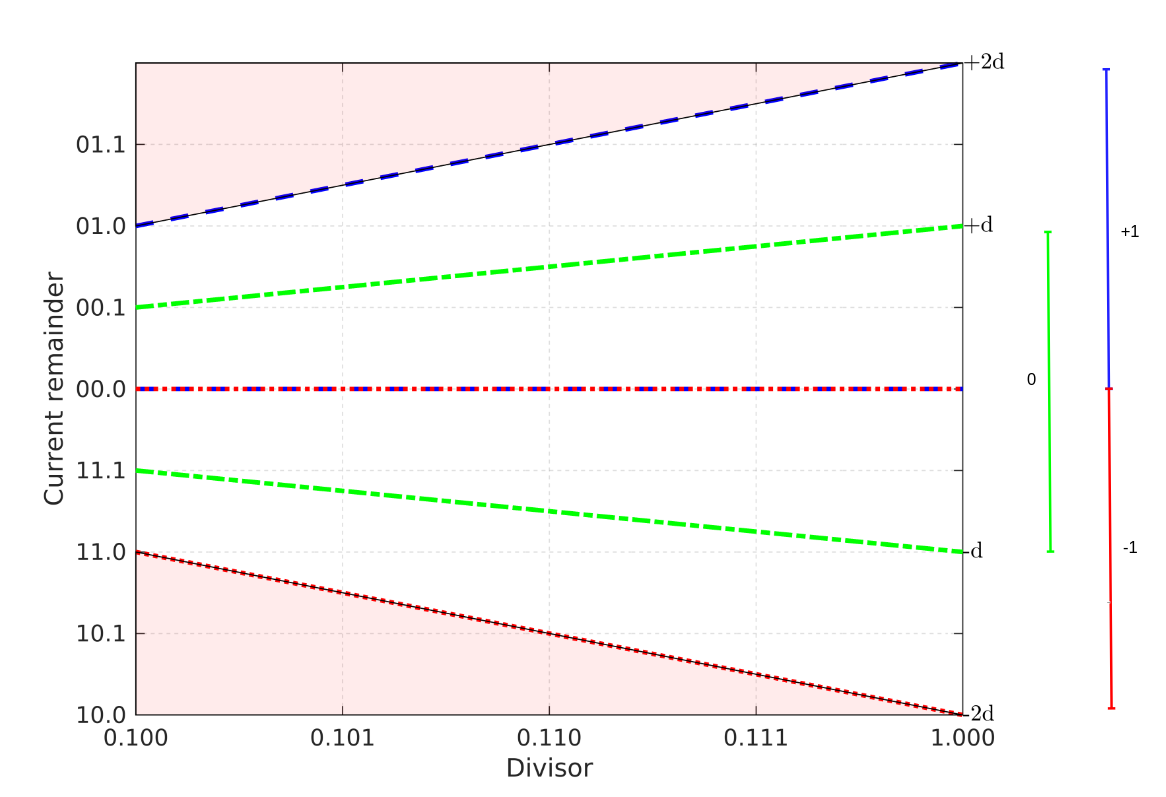
\includegraphics[width=100mm]{images/pd_plot_r2.png}
    \caption{p-d plot for SRT radix-2}
    \label{fig:pd_radix_2}
\end{figure}

Once $q_i$ has been chosen, the algorithm computes the next remainder as $A_{i+1} = 2\cdot (A_i - q_i\cdot d \cdot 2^{N/2})$. 
Regarding the representation of the quotient, there are many possible ways to store it.
It can be stored in the standard binary representation by computing the translation from the $\{-1, 0, 1\}$ digit set \textit{on the fly}, without the need to go back to a $\{0, 1\}$ digit set at the end of the algorithm. 
This \textit{on the fly} conversion is performed at each step by computing $Q = 2\cdot Q + q_i$. 
From an implementation point of view, this is means having the possibility to sum or subtract one to the shifted current quotient.

Before introducing the code, we need to cover one last element: the normalisation of the input values. 
In order to have the divisor in the range $[\frac{1}{2}, 1)$, we need to remove all the leading zeros, which means \textit{shifting left as many times as the number of leading zeroes}. 
From an hardware point of view, this operation can be performed with a barrel shifter and a combinational circuit to detect the number of leading zeros $k$. 
Once we have shifted the divisor, we apply the same left shift to the dividend: after this normalisation the final quotient will be correct but to get the correct remainder we will need to shift it to the right by $k$ positions (the quotient is unsigned so we would push zeroes as most significant bits). 

Here is a the code to execute this algorithm.
The function \texttt{srt\_division\_radix\_
2\_lut} implements \autoref{tab:srt_radix2}. 

\begin{lstlisting}[language=C++]
std::pair<SLV::std_logic_vector, SLV::std_logic_vector> 
Division::srt_division_radix_2
(SLV::std_logic_vector& dividend, SLV::std_logic_vector & divisor){
    
    int N = divisor.size;

    if(dividend.to_base_10() >= (divisor.to_base_10() << N/2)
        throw std::invalid_argument();
 
    SLV::std_logic_vector A (N   + 2);
    SLV::std_logic_vector B (N/2 + 2);
    SLV::std_logic_vector Q (N/2 + 2);

    unsigned int k = 
        divisor.extract(N/2 - 1, 0).count_leading_zeros();

    A = SLV::std_logic_vector("00") & (dividend << k);
    B = SLV::std_logic_vector("00") & (divisor.extract(N/2 - 1, 0) << k);
 
    for(int i = 0; i <= N/2; i++){
        SLV::std_logic_vector A_upper  = 
            A.extract(N + 1, N/2);
        SLV::std_logic_vector A_bottom = 
            A.extract(N/2 - 1, 0);
        SLV::std_logic_vector A_top    = 
            A.extract(N + 1, N - 1);

        SLV::std_logic_vector partial_R(N/2 + 2);

        int current_q =
            srt_division_radix_2_lut(A_top);

        if(current_q == 0)
            Q =  (Q << 1),
            partial_R = A_upper;

        if(current_q == 1)
            Q = ((Q << 1) + 1),
            partial_R = A_upper - B;

        if(current_q == -1)
            Q = ((Q << 1) - 1),
            partial_R = A_upper + B;
            
        A = (partial_R & A_bottom) << 1;
    }

    if(A.get_msb()){
        Q = Q - 1;
        A = A >> 1;
        A = (A.extract(N + 1, N/2) + B) & A.extract(N/2 - 1, 0);
        A = A << 1;
    }

    SLV::std_logic_vector R = A.extract(N + 1, N/2 + 1) >> k;
    Q = Q.extract(N/2 - 1, 0);

    return std::pair<SLV::std_logic_vector, SLV::std_logic_vector>
    (Q, R);
} 
\end{lstlisting}

As it was for the non restoring algorithm, after the iterations are completed we may end up with a negative remainder: in this case we decrease $Q$ by 1 and correct $A$. 

\begin{figure}
    \centering
    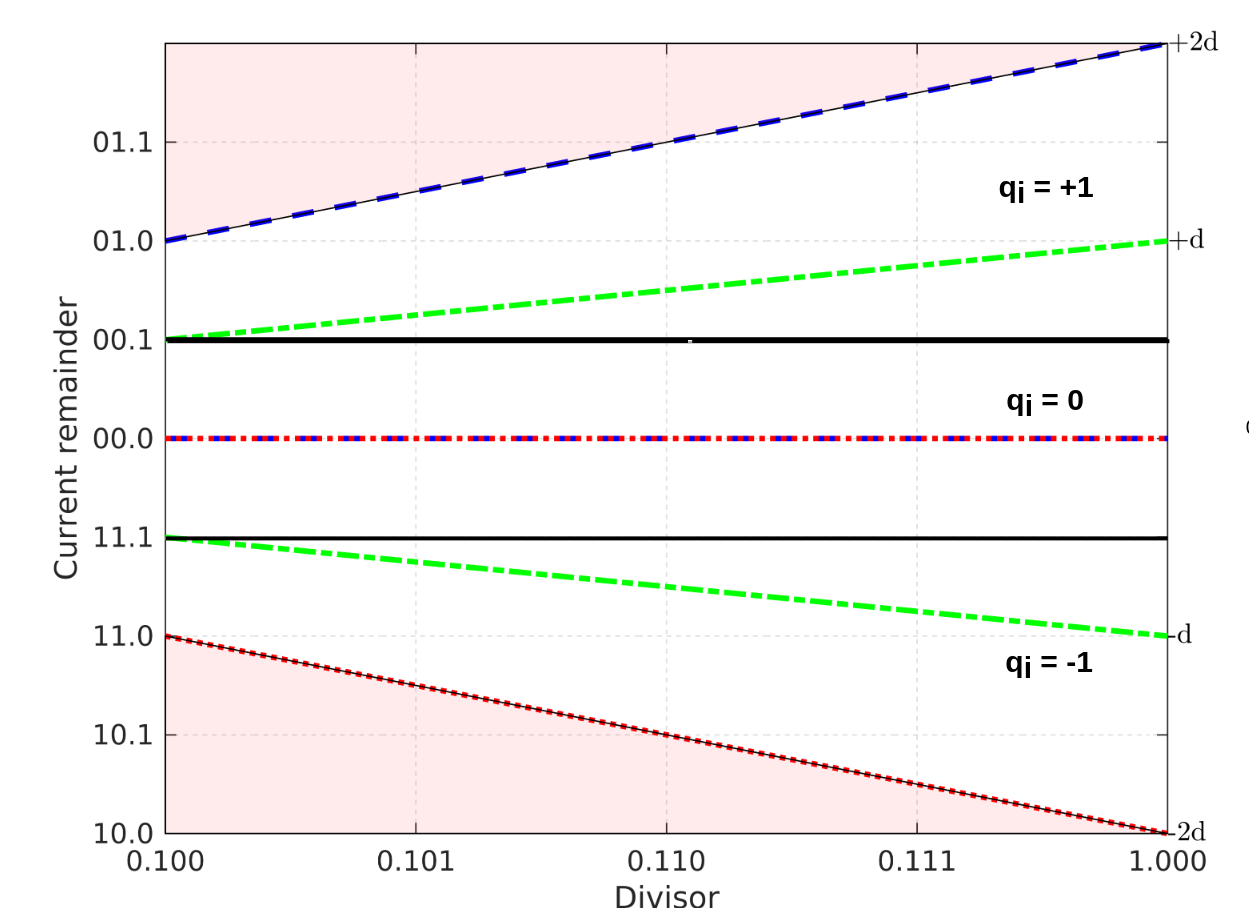
\includegraphics[width=100mm]{images/pd_plot_r2_q.png}
    \caption{p-d plot for radix 2 showing the boundaries to select the digits}
    \label{fig:pd_radix_2_dig}
\end{figure}

\subsection{Radix-4 algorithm}
Once that we have understood how does the radix-2 algorithm works, it is easy to apply the same concepts to higher radixes. 
The radix-4 implementation is able to compute 2 digits of the quotient ad a time: in order to do so, the digit set of the quotient can either be $\{-3, -2, -1, 0, +1, +2, +3\}$ (called \textit{maximally redundant digit set}) or $\{-2, -1, 0, +1, +2\}$ (called \textit{minimally redundant digit set}). 
None of them is unconditionally better than the other: the \textit{maximally redundant} set  has a small look-up table with $2^5=32$ entries, but the required hardware to perform the computations is more complex; the \textit{minimally redundant} set is simpler to implement, but the look-up table has $2^9=512$ entries. 

Our final implementation of the circuit uses the \textit{minimally redundant} digit set: at each step of the loop, once we have chosen the $q_i$ digit, what we need to do is compute $Q_{i+1} = 4 \cdot Q_i + q_i$ and $A_{i+1} = 4 \cdot (A_i - q_i \cdot d \cdot 2^n)$.

The main problem is coming up with the look up table, but again the \textit{p-d} plot can be used for that purpose. 
First of all we need to define it, then we need to set the boundaries to use for the digit selection and then we use all this information to extract a look up table. 

We want the partial remainder for a given iteration $i$ to be in $[-hd, hd]$ (with $h$ being a scaling factor), while the remainder produced by the previous iteration is in $[-4hd, 4hd]$ due to the fact that it was shifted left by two positions. 
Since at most we can add or subtract $2d$ to that remainder, we need to satisfy:
\[
    4hd - 2d \ge hd \Rightarrow h \le \frac{2}{3}
\]

If we choose $h = \frac{2}{3}$, we can compute the limits of each digit selection interval the following way: 
\begin{align*} 
2_{upper} &= +\frac{2}{3}\cdot d + 2 \cdot d = +\frac{8}{3}\cdot d \\
2_{lower} &= -\frac{2}{3}\cdot d + 2 \cdot d = +\frac{4}{3}\cdot d \\
1_{upper} &= +\frac{2}{3}\cdot d + 1 \cdot d = +\frac{5}{3}\cdot d \\
1_{lower} &= -\frac{2}{3}\cdot d + 1 \cdot d = +\frac{1}{3}\cdot d\\
0_{upper} &= +\frac{2}{2}\cdot d + 0 \cdot d= +\frac{2}{3}\cdot d  \\
0_{lower} &= -\frac{2}{3} \cdot d - 0 \cdot d = -\frac{2}{3} \cdot d\\
-1_{upper} &= +\frac{2}{3}\cdot d - 1 \cdot d = -\frac{1}{3}\cdot d \\
-1_{lower} &= -\frac{2}{3}\cdot d - 1 \cdot d = -\frac{5}{3}\cdot d \\
-2_{upper} &= +\frac{2}{3}\cdot d - 2 \cdot d = -\frac{4}{3}\cdot d \\
-2_{lower} &= -\frac{2}{3}\cdot d - 2 \cdot d = -\frac{8}{3}\cdot d \\
\end{align*}

\begin{figure}
    \centering
    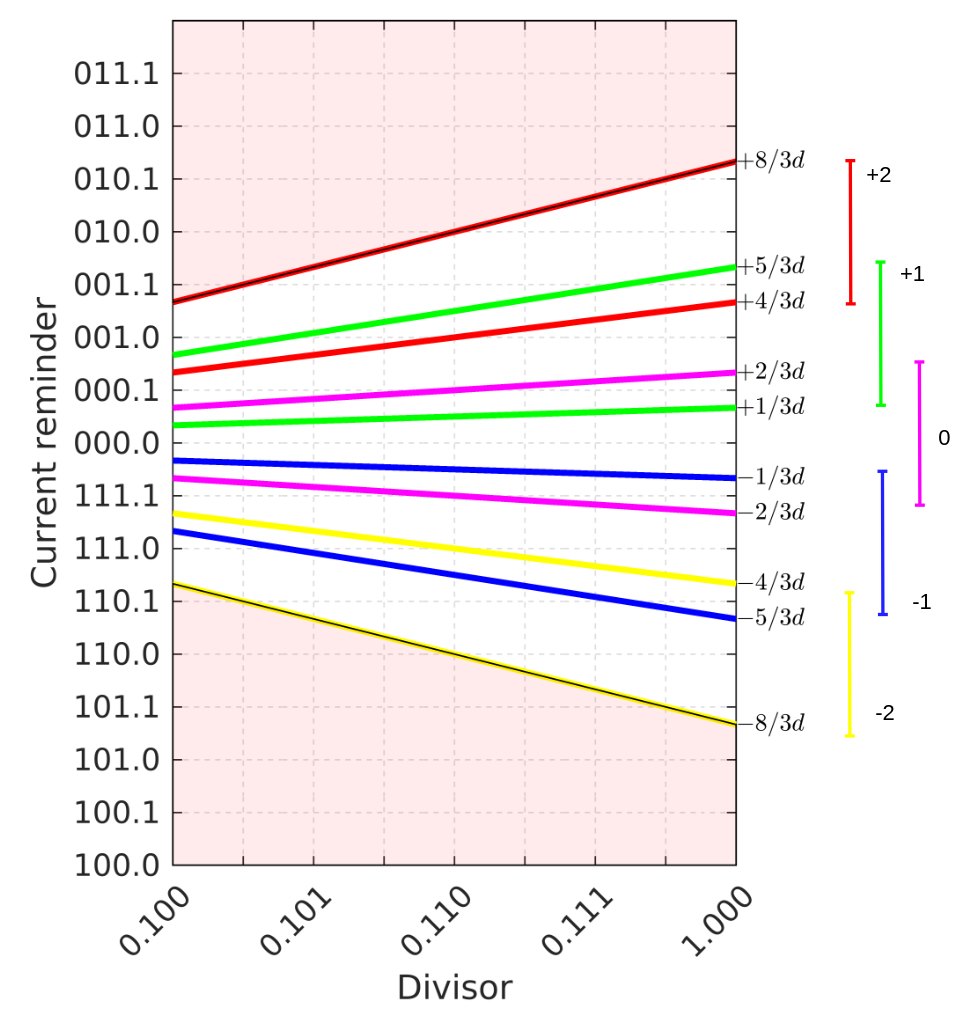
\includegraphics[width=100mm]{images/pd_plot_r4.png}
    \caption{p-d plot for SRT radix-4, with minimum binary set}
    \label{fig:pd_radix_4}
\end{figure}

Thanks to these values, we end up with the plot in \autoref{fig:pd_radix_4}, whose structure is the same as the one of \autoref{fig:pd_radix_2}, which was previously defined.  

The regions associated with each digit cannot be delimited using horizontal lines, which means that we need to take into account the digits of the divisor $d$ as well as those of $A$ and that the boundaries are now broken lines. 
We can thus partition the plot, and associate  a digit of the quotient to each partition. 
This is what is done in \autoref{fig:pd_radix_4_dig}, using the black lines as boundaries. 
Thanks to this separation, it is possible to build the look-up table using as inputs 6 digits from $A$ and 3 digits from $d$. 
Since there is no available look-up table on the internet for this algorithm, radix and digit set, its declaration can be found in its entirety in \autoref{tab:srt_radix4}.
Using these few principles, we can come up with an SRT division algorithm with radix $2^k$. 

\begin{figure}
    \centering
    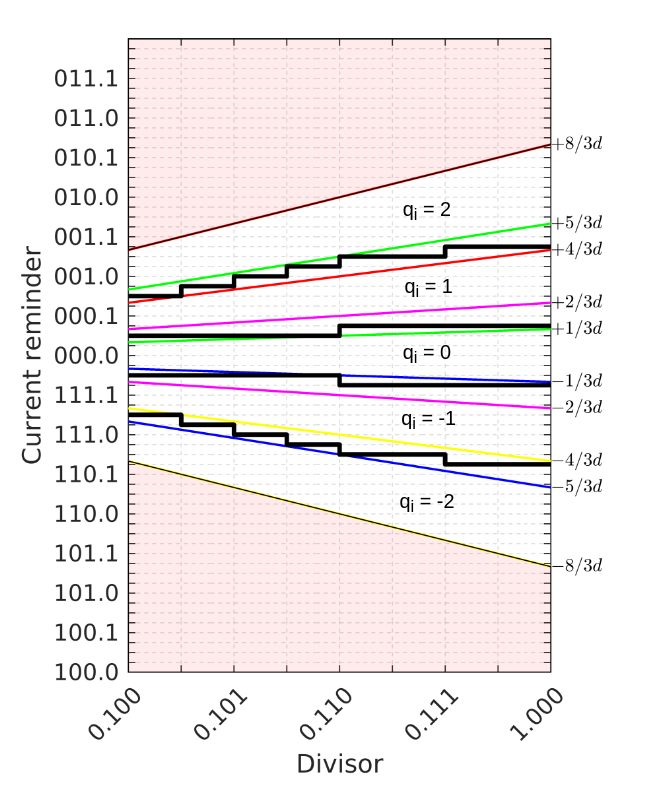
\includegraphics[width=100mm]{images/pd_plot_r4_q.png}
    \caption{p-d plot for radix 4 showing the boundaries to select the digits}
    \label{fig:pd_radix_4_dig}
\end{figure}

As it happened in the previous case, the areas above $\frac{8}{3}\cdot d$ and below $-\frac{8}{3}\cdot d$ are not feasible, due to the constraints we put on the operands. In spite of that, we still need to insert the points in those areas in the look-up table and associate them to $q_i = 2$ or $q_i = -2$, respectively.
The code which implements this algorithm can be found in \autoref{Chapter_Impl_Div}, since it is fundamental to understand the structure of the division circuit. 

Now we have all the knowledge to understand what happened in the Pentium division unit in 1990 \cite{10.1007/3-540-59293-8_189}: Intel used a radix-4 SRT division with a look-up table similar to the one presented.
However, while defining this table using the p-d plot, the boundaries were computed incorrectly and some areas were associated to the wrong digits: when an $(A, d)$ couple belonged to these areas, the result ended up being incorrect.
These issues had not been discovered during the verification of the chip due to fact that the probability of using these incorrect entries was very low (one in ten billion).
Regardless, the problem was noticed by the users and Intel had to pay \$475 million  to recall the defective processors and fix the issue. 

\begin{table}
  \begin{center}
    \small
    \caption{Possible look up table for radix-4 SRT using minimally redundant digit set $\{-2, -1, 0, +1, +2\}$}
    \label{tab:srt_radix4}
    \scalebox{0.6}{
    \begin{tabular}{||c|c|c||c|c|c||c|c|c||c|c|c||c|c|c||c|c|c||c|c|c||c|c|c||} 
        \hline
        $B$ & $A$ & $q_i$ & $B$ & $A$ & $q_i$ & $B$ & $A$ & $q_i$ & $B$ & $A$ & $q_i$ & $B$ & $A$ & $q_i$ & $B$ & $A$ & $q_i$ & $B$ & $A$ & $q_i$ & $B$ & $A$ & $q_i$ \\
        \hline
000 & 000000 & 0 & 001 & 000000 & 0 & 010 & 000000 & 0 & 011 & 000000 & 0 & 100 & 000000 & 0 & 101 & 000000 & 0 & 110 & 000000 & 0 & 111 & 000000 & 0\\
000 & 000001 & 0 & 001 & 000001 & 0 & 010 & 000001 & 0 & 011 & 000001 & 0 & 100 & 000001 & 0 & 101 & 000001 & 0 & 110 & 000001 & 0 & 111 & 000001 & 0\\
000 & 000010 & 1 & 001 & 000010 & 1 & 010 & 000010 & 1 & 011 & 000010 & 1 & 100 & 000010 & 0 & 101 & 000010 & 0 & 110 & 000010 & 0 & 111 & 000010 & 0\\
000 & 000011 & 1 & 001 & 000011 & 1 & 010 & 000011 & 1 & 011 & 000011 & 1 & 100 & 000011 & 1 & 101 & 000011 & 1 & 110 & 000011 & 1 & 111 & 000011 & 1\\
000 & 000100 & 1 & 001 & 000100 & 1 & 010 & 000100 & 1 & 011 & 000100 & 1 & 100 & 000100 & 1 & 101 & 000100 & 1 & 110 & 000100 & 1 & 111 & 000100 & 1\\
000 & 000101 & 1 & 001 & 000101 & 1 & 010 & 000101 & 1 & 011 & 000101 & 1 & 100 & 000101 & 1 & 101 & 000101 & 1 & 110 & 000101 & 1 & 111 & 000101 & 1\\
000 & 000110 & 2 & 001 & 000110 & 1 & 010 & 000110 & 1 & 011 & 000110 & 1 & 100 & 000110 & 1 & 101 & 000110 & 1 & 110 & 000110 & 1 & 111 & 000110 & 1\\
000 & 000111 & 2 & 001 & 000111 & 2 & 010 & 000111 & 1 & 011 & 000111 & 1 & 100 & 000111 & 1 & 101 & 000111 & 1 & 110 & 000111 & 1 & 111 & 000111 & 1\\
000 & 001000 & 2 & 001 & 001000 & 2 & 010 & 001000 & 2 & 011 & 001000 & 1 & 100 & 001000 & 1 & 101 & 001000 & 1 & 110 & 001000 & 1 & 111 & 001000 & 1\\
000 & 001001 & 2 & 001 & 001001 & 2 & 010 & 001001 & 2 & 011 & 001001 & 2 & 100 & 001001 & 1 & 101 & 001001 & 1 & 110 & 001001 & 1 & 111 & 001001 & 1\\
000 & 001010 & 2 & 001 & 001010 & 2 & 010 & 001010 & 2 & 011 & 001010 & 2 & 100 & 001010 & 2 & 101 & 001010 & 2 & 110 & 001010 & 1 & 111 & 001010 & 1\\
000 & 001011 & 2 & 001 & 001011 & 2 & 010 & 001011 & 2 & 011 & 001011 & 2 & 100 & 001011 & 2 & 101 & 001011 & 2 & 110 & 001011 & 2 & 111 & 001011 & 2\\
000 & 001100 & 2 & 001 & 001100 & 2 & 010 & 001100 & 2 & 011 & 001100 & 2 & 100 & 001100 & 2 & 101 & 001100 & 2 & 110 & 001100 & 2 & 111 & 001100 & 2\\
000 & 001101 & 2 & 001 & 001101 & 2 & 010 & 001101 & 2 & 011 & 001101 & 2 & 100 & 001101 & 2 & 101 & 001101 & 2 & 110 & 001101 & 2 & 111 & 001101 & 2\\
000 & 001110 & 2 & 001 & 001110 & 2 & 010 & 001110 & 2 & 011 & 001110 & 2 & 100 & 001110 & 2 & 101 & 001110 & 2 & 110 & 001110 & 2 & 111 & 001110 & 2\\
000 & 001111 & 2 & 001 & 001111 & 2 & 010 & 001111 & 2 & 011 & 001111 & 2 & 100 & 001111 & 2 & 101 & 001111 & 2 & 110 & 001111 & 2 & 111 & 001111 & 2\\
000 & 010000 & 2 & 001 & 010000 & 2 & 010 & 010000 & 2 & 011 & 010000 & 2 & 100 & 010000 & 2 & 101 & 010000 & 2 & 110 & 010000 & 2 & 111 & 010000 & 2\\
000 & 010001 & 2 & 001 & 010001 & 2 & 010 & 010001 & 2 & 011 & 010001 & 2 & 100 & 010001 & 2 & 101 & 010001 & 2 & 110 & 010001 & 2 & 111 & 010001 & 2\\
000 & 010010 & 2 & 001 & 010010 & 2 & 010 & 010010 & 2 & 011 & 010010 & 2 & 100 & 010010 & 2 & 101 & 010010 & 2 & 110 & 010010 & 2 & 111 & 010010 & 2\\
000 & 010011 & 2 & 001 & 010011 & 2 & 010 & 010011 & 2 & 011 & 010011 & 2 & 100 & 010011 & 2 & 101 & 010011 & 2 & 110 & 010011 & 2 & 111 & 010011 & 2\\
000 & 010100 & 2 & 001 & 010100 & 2 & 010 & 010100 & 2 & 011 & 010100 & 2 & 100 & 010100 & 2 & 101 & 010100 & 2 & 110 & 010100 & 2 & 111 & 010100 & 2\\
000 & 010101 & 2 & 001 & 010101 & 2 & 010 & 010101 & 2 & 011 & 010101 & 2 & 100 & 010101 & 2 & 101 & 010101 & 2 & 110 & 010101 & 2 & 111 & 010101 & 2\\
000 & 010110 & 2 & 001 & 010110 & 2 & 010 & 010110 & 2 & 011 & 010110 & 2 & 100 & 010110 & 2 & 101 & 010110 & 2 & 110 & 010110 & 2 & 111 & 010110 & 2\\
000 & 010111 & 2 & 001 & 010111 & 2 & 010 & 010111 & 2 & 011 & 010111 & 2 & 100 & 010111 & 2 & 101 & 010111 & 2 & 110 & 010111 & 2 & 111 & 010111 & 2\\
000 & 011000 & 2 & 001 & 011000 & 2 & 010 & 011000 & 2 & 011 & 011000 & 2 & 100 & 011000 & 2 & 101 & 011000 & 2 & 110 & 011000 & 2 & 111 & 011000 & 2\\
000 & 011001 & 2 & 001 & 011001 & 2 & 010 & 011001 & 2 & 011 & 011001 & 2 & 100 & 011001 & 2 & 101 & 011001 & 2 & 110 & 011001 & 2 & 111 & 011001 & 2\\
000 & 011010 & 2 & 001 & 011010 & 2 & 010 & 011010 & 2 & 011 & 011010 & 2 & 100 & 011010 & 2 & 101 & 011010 & 2 & 110 & 011010 & 2 & 111 & 011010 & 2\\
000 & 011011 & 2 & 001 & 011011 & 2 & 010 & 011011 & 2 & 011 & 011011 & 2 & 100 & 011011 & 2 & 101 & 011011 & 2 & 110 & 011011 & 2 & 111 & 011011 & 2\\
000 & 011100 & 2 & 001 & 011100 & 2 & 010 & 011100 & 2 & 011 & 011100 & 2 & 100 & 011100 & 2 & 101 & 011100 & 2 & 110 & 011100 & 2 & 111 & 011100 & 2\\
000 & 011101 & 2 & 001 & 011101 & 2 & 010 & 011101 & 2 & 011 & 011101 & 2 & 100 & 011101 & 2 & 101 & 011101 & 2 & 110 & 011101 & 2 & 111 & 011101 & 2\\
000 & 011110 & 2 & 001 & 011110 & 2 & 010 & 011110 & 2 & 011 & 011110 & 2 & 100 & 011110 & 2 & 101 & 011110 & 2 & 110 & 011110 & 2 & 111 & 011110 & 2\\
000 & 011111 & 2 & 001 & 011111 & 2 & 010 & 011111 & 2 & 011 & 011111 & 2 & 100 & 011111 & 2 & 101 & 011111 & 2 & 110 & 011111 & 2 & 111 & 011111 & 2\\
000 & 100000 & -2 & 001 & 100000 & -2 & 010 & 100000 & -2 & 011 & 100000 & -2 & 100 & 100000 & -2 & 101 & 100000 & -2 & 110 & 100000 & -2 & 111 & 100000 & -2\\
000 & 100001 & -2 & 001 & 100001 & -2 & 010 & 100001 & -2 & 011 & 100001 & -2 & 100 & 100001 & -2 & 101 & 100001 & -2 & 110 & 100001 & -2 & 111 & 100001 & -2\\
000 & 100010 & -2 & 001 & 100010 & -2 & 010 & 100010 & -2 & 011 & 100010 & -2 & 100 & 100010 & -2 & 101 & 100010 & -2 & 110 & 100010 & -2 & 111 & 100010 & -2\\
000 & 100011 & -2 & 001 & 100011 & -2 & 010 & 100011 & -2 & 011 & 100011 & -2 & 100 & 100011 & -2 & 101 & 100011 & -2 & 110 & 100011 & -2 & 111 & 100011 & -2\\
000 & 100100 & -2 & 001 & 100100 & -2 & 010 & 100100 & -2 & 011 & 100100 & -2 & 100 & 100100 & -2 & 101 & 100100 & -2 & 110 & 100100 & -2 & 111 & 100100 & -2\\
000 & 100101 & -2 & 001 & 100101 & -2 & 010 & 100101 & -2 & 011 & 100101 & -2 & 100 & 100101 & -2 & 101 & 100101 & -2 & 110 & 100101 & -2 & 111 & 100101 & -2\\
000 & 100110 & -2 & 001 & 100110 & -2 & 010 & 100110 & -2 & 011 & 100110 & -2 & 100 & 100110 & -2 & 101 & 100110 & -2 & 110 & 100110 & -2 & 111 & 100110 & -2\\
000 & 100111 & -2 & 001 & 100111 & -2 & 010 & 100111 & -2 & 011 & 100111 & -2 & 100 & 100111 & -2 & 101 & 100111 & -2 & 110 & 100111 & -2 & 111 & 100111 & -2\\
000 & 101000 & -2 & 001 & 101000 & -2 & 010 & 101000 & -2 & 011 & 101000 & -2 & 100 & 101000 & -2 & 101 & 101000 & -2 & 110 & 101000 & -2 & 111 & 101000 & -2\\
000 & 101001 & -2 & 001 & 101001 & -2 & 010 & 101001 & -2 & 011 & 101001 & -2 & 100 & 101001 & -2 & 101 & 101001 & -2 & 110 & 101001 & -2 & 111 & 101001 & -2\\
000 & 101010 & -2 & 001 & 101010 & -2 & 010 & 101010 & -2 & 011 & 101010 & -2 & 100 & 101010 & -2 & 101 & 101010 & -2 & 110 & 101010 & -2 & 111 & 101010 & -2\\
000 & 101011 & -2 & 001 & 101011 & -2 & 010 & 101011 & -2 & 011 & 101011 & -2 & 100 & 101011 & -2 & 101 & 101011 & -2 & 110 & 101011 & -2 & 111 & 101011 & -2\\
000 & 101100 & -2 & 001 & 101100 & -2 & 010 & 101100 & -2 & 011 & 101100 & -2 & 100 & 101100 & -2 & 101 & 101100 & -2 & 110 & 101100 & -2 & 111 & 101100 & -2\\
000 & 101101 & -2 & 001 & 101101 & -2 & 010 & 101101 & -2 & 011 & 101101 & -2 & 100 & 101101 & -2 & 101 & 101101 & -2 & 110 & 101101 & -2 & 111 & 101101 & -2\\
000 & 101110 & -2 & 001 & 101110 & -2 & 010 & 101110 & -2 & 011 & 101110 & -2 & 100 & 101110 & -2 & 101 & 101110 & -2 & 110 & 101110 & -2 & 111 & 101110 & -2\\
000 & 101111 & -2 & 001 & 101111 & -2 & 010 & 101111 & -2 & 011 & 101111 & -2 & 100 & 101111 & -2 & 101 & 101111 & -2 & 110 & 101111 & -2 & 111 & 101111 & -2\\
000 & 110000 & -2 & 001 & 110000 & -2 & 010 & 110000 & -2 & 011 & 110000 & -2 & 100 & 110000 & -2 & 101 & 110000 & -2 & 110 & 110000 & -2 & 111 & 110000 & -2\\
000 & 110001 & -2 & 001 & 110001 & -2 & 010 & 110001 & -2 & 011 & 110001 & -2 & 100 & 110001 & -2 & 101 & 110001 & -2 & 110 & 110001 & -2 & 111 & 110001 & -2\\
000 & 110010 & -2 & 001 & 110010 & -2 & 010 & 110010 & -2 & 011 & 110010 & -2 & 100 & 110010 & -2 & 101 & 110010 & -2 & 110 & 110010 & -2 & 111 & 110010 & -2\\
000 & 110011 & -2 & 001 & 110011 & -2 & 010 & 110011 & -2 & 011 & 110011 & -2 & 100 & 110011 & -2 & 101 & 110011 & -2 & 110 & 110011 & -2 & 111 & 110011 & -2\\
000 & 110100 & -2 & 001 & 110100 & -2 & 010 & 110100 & -2 & 011 & 110100 & -2 & 100 & 110100 & -2 & 101 & 110100 & -2 & 110 & 110100 & -2 & 111 & 110100 & -2\\
000 & 110101 & -2 & 001 & 110101 & -2 & 010 & 110101 & -2 & 011 & 110101 & -2 & 100 & 110101 & -2 & 101 & 110101 & -2 & 110 & 110101 & -1 & 111 & 110101 & -1\\
000 & 110110 & -2 & 001 & 110110 & -2 & 010 & 110110 & -2 & 011 & 110110 & -2 & 100 & 110110 & -1 & 101 & 110110 & -1 & 110 & 110110 & -1 & 111 & 110110 & -1\\
000 & 110111 & -2 & 001 & 110111 & -2 & 010 & 110111 & -2 & 011 & 110111 & -1 & 100 & 110111 & -1 & 101 & 110111 & -1 & 110 & 110111 & -1 & 111 & 110111 & -1\\
000 & 111000 & -2 & 001 & 111000 & -2 & 010 & 111000 & -1 & 011 & 111000 & -1 & 100 & 111000 & -1 & 101 & 111000 & -1 & 110 & 111000 & -1 & 111 & 111000 & -1\\
000 & 111001 & -2 & 001 & 111001 & -1 & 010 & 111001 & -1 & 011 & 111001 & -1 & 100 & 111001 & -1 & 101 & 111001 & -1 & 110 & 111001 & -1 & 111 & 111001 & -1\\
000 & 111010 & -1 & 001 & 111010 & -1 & 010 & 111010 & -1 & 011 & 111010 & -1 & 100 & 111010 & -1 & 101 & 111010 & -1 & 110 & 111010 & -1 & 111 & 111010 & -1\\
000 & 111011 & -1 & 001 & 111011 & -1 & 010 & 111011 & -1 & 011 & 111011 & -1 & 100 & 111011 & -1 & 101 & 111011 & -1 & 110 & 111011 & -1 & 111 & 111011 & -1\\
000 & 111100 & -1 & 001 & 111100 & -1 & 010 & 111100 & -1 & 011 & 111100 & -1 & 100 & 111100 & -1 & 101 & 111100 & -1 & 110 & 111100 & -1 & 111 & 111100 & -1\\
000 & 111101 & -1 & 001 & 111101 & -1 & 010 & 111101 & -1 & 011 & 111101 & -1 & 100 & 111101 & 0 & 101 & 111101 & 0 & 110 & 111101 & 0 & 111 & 111101 & 0\\
000 & 111110 & 0 & 001 & 111110 & 0 & 010 & 111110 & 0 & 011 & 111110 & 0 & 100 & 111110 & 0 & 101 & 111110 & 0 & 110 & 111110 & 0 & 111 & 111110 & 0\\
000 & 111111 & 0 & 001 & 111111 & 0 & 010 & 111111 & 0 & 011 & 111111 & 0 & 100 & 111111 & 0 & 101 & 111111 & 0 & 110 & 111111 & 0 & 111 & 111111 & 0\\
        \hline
    \end{tabular}}
  \end{center}
\end{table}